\section{Marco teórico de referencia y antecedentes}

El marco de referencia está organizado en un primer momento con el análisis del estado del arte para la comprensión del objeto de estudios sobre MLOps para el ámbito agrícola y un segundo momento con los elementos teórico-conceptuales que permiten la argumentación teórica sobre Machine Learning, la metodología MLOps y el cultivo de aguacate Hass con las plagas detalladas para esta investigación.

\subsection{Estado del arte}
Las investigaciones a nivel internacional se describen a continuación

\begin{longtable}{|p{2cm}|p{3cm}|p{3cm}|p{4cm}|p{3cm}|}

\caption{Investigaciones internacionales}\\
\hline
\textbf{Autor} & \textbf{Título} & \textbf{Objetivo} & \textbf{Metodología} & \textbf{Resultado} \\
\hline
\endhead

\citet{aimacana2021} & Análisis comparativo de algoritmos de Machine Learning para la detección de plagas en los cultivos representativos de la sierra ecuatoriana & Realizar un análisis comparativo entre distintos algoritmos de Machine y Deep Learning, que permita determinar cuál de ellos ofrece mejores resultados en la detección de plagas en cultivos endémicos de la serranía ecuatoriana. & Metodología CRISPDM la cual sus siglas significan Proceso Estándar Entre Industrias para la Minería de Datos. & El estudio realizado se aplicó el mejor modelo para la construcción de un prototipo el cual fue la red neuronal convolucional InceptionV3; el prototipo realizado, permite al usuario enviar imágenes para ser procesadas por el modelo y este a su vez reciba una predicción he información de los síntomas, además de una sugerencia de un posible tratamiento. \\
\hline
\citet{castaneda2021} & Detección de nutrientes del suelo y planta, y pestes en campos de cultivo de banano orgánico con Machine Learning & Diseño una plataforma que sirva de apoyo al agricultor para poder estimar qué macronutrientes tiene en deficiencia su planta de banano, con la finalidad de obtener un mejor producto en la cosecha del banano orgánico, así como una posible interfaz para la detección de plagas en el banano. & Se utilizó un conjunto de fotografías público, el cual fue encontrado en un repositorio y se escogieron aquellas plagas que afectaban al banano. Posteriormente, se realizó un aumento a este conjunto de fotografías mediante transformaciones lineales y las imágenes resultantes fueron pre procesadas en diferentes espacios de color para ser utilizadas como entradas a la red neuronal. & El modelo permitió una alta precisión a través de diferentes métricas. Continuamente se desarrolló un prototipo de plataforma web para que los agricultores en un futuro pudieran acceder al sistema. \\
\hline
\citet{valenzuela2022} & Detección y Clasificación de Enfermedades en el Tomate Mediante Deep Learning y Computer Visión & Aplicar el aprendizaje profundo a problemas de visión de computadora tales como detección y clasificación específicamente en las enfermedades del tomate mediante el procesamiento de imágenes digitales. & Neuronales pre-entrenadas (transfer learning), para hacer la detección de la hoja de tomate (primera: Faster Mask R-CNN) y luego a partir de la detección, realizar la clasificación de la enfermedad (segunda: red neuronal convolucional), tomando como entrada el área de la imagen donde se encuentra la hoja, luego de realizar la clasificación el sistema desarrollado proporciona información de los síntomas asociados a la enfermedad, como también cómo proceder con la prevención y el tratamiento a seguir en tiempo real. & Con el advenimiento de las redes neuronales, ha permitido mejorar drásticamente la precisión, tanto de la detección de objetos como de la clasificación de imágenes. \\
\hline
\citet{garcia2022} & Implementación de modelo Machine Learning aplicado al estudio de enfermedades de café en el centro de investigación Sacha Wiwa, perteneciente a la parroquia Gasaganga, Cantón la Maná, provincia de Cotopaxi & Implementar modelo de clasificación de imágenes empleando técnicas de Machine Learning, para la detección de enfermedades del Cafeto (Coffea arábica) en huertas del Centro de Investigación Sacha Wiwa. & Cualitativa experimental permite la selección, análisis y presentación de los datos documentados de una manera ordenada y siguiendo los objetivos del proyecto. & Mediante el modelo de Machine Learning desarrollado en el entorno virtual “Jupyter lab” se logró crear y entrenar las redes neuronales convencionales para la clasificación de las enfermedades del café expuestas en el caso de estudio en conjunto con la clasificación sana del cafeto. \\
\hline
\caption*{\footnotesize Fuente: Elaboración del investigador}
\end{longtable}


En las investigaciones a nivel internacional se pude observar que el desarrollo de Machine Learning, en particular el uso de redes neuronales, ha demostrado ser de gran importancia en el control de plagas y enfermedades en diversos campos, como la agricultura, asimismo este utiliza un modelo de red neuronal convolucional para la detección de plagas y enfermedades como por ejemplo en los cultivos de  café,  tomate y banano donde es un ejemplo claro de cómo el Machine Learning puede contribuir al control de plagas.

Uno de los principales beneficios del Machine Learning en el control de plagas es su capacidad para analizar grandes volúmenes de datos y extraer patrones y características relevantes, en las investigaciones se observaron que utilizaban imágenes  de plantas enfermas como sanas, lo que le permitió aprender a reconocer los síntomas y distinguir entre diferentes enfermedades. Esto es especialmente útil en el control de plagas, ya que puede facilitar la detección temprana de enfermedades y ayudar a los agricultores a tomar medidas preventivas o correctivas de manera oportuna.

Para el caso de las investigaciones nacionales se detallan en la siguiente tabla:


\begin{longtable}{|p{2cm}|p{3cm}|p{3cm}|p{4cm}|p{3cm}|}

\caption{Investigaciones a nivel nacional}\\
\hline
\textbf{Autor} & \textbf{Título} & \textbf{Objetivo} & \textbf{Metodología} & \textbf{Resultado} \\
\hline
\endhead

\hline
\endfoot

\hline
\endlastfoot

\citet{tovar2019} & Diseño e implementación de un aplicativo móvil para realizar la detección temprana de la enfermedad de la Sigatoka Negra en los cultivos de plátanos & Diseñar e implementar un aplicativo móvil, para realizar la detección temprana de la enfermedad de la Sigatoka Negra en los cultivos de plátanos. & La metodología utilizada para la detección de esta enfermedad, consistió en construir una base de datos que contiene imágenes de los posibles estados de la misma, teniendo en cuenta la escala estándar de Fouré utilizada para analizar la forma de evolución de la Sigatoka Negra. Luego se inició con la creación del algoritmo, en donde se realizó la segmentación de cada una de las imágenes para generar un realce en la enfermedad, para posteriormente obtener las características respectivas y finalmente a partir de las técnicas de Machine Learning generar una clasificación que identifique el estadío en el que se encuentra una hoja al tomar una imagen que no se ubique dentro de la base de datos. & El aplicativo móvil demostró un porcentaje de acierto del 80\% en la detección de la Sigatoka Negra. Por lo tanto, la aplicación puede llegar a ayudar a los productores de plátano, evitando así pérdidas económicas. \\
\citet{avila2022} & Entrenamiento de redes neuronales para la identificación de plagas en cultivos de café. & Implementar un aplicativo basado en visión artificial para la identificación de Cercospora, Phoma, Roya, minador de hojas y Arañita roja, en el café a partir del análisis de las hojas de la planta. & Esta base será introducida a modelos de redes neuronales: densa, neuronal convolucional y neuronal convolucional con overfitting, usando el lenguaje Python y las bibliotecas: Keras y TensorFlow. Una vez entrenado el modelo, se procede al análisis de las imágenes que contienen la morfología de la planta y que servirán de entrada a una red neuronal para poder comparar los resultados y determinar cuál de los modelos presenta mejores resultados. & El modelo convolucional con overfitting presenta el mejor resultado de predicción, pero aun así, es un modelo limitado que podría ser reemplazado por otros modelos de mayor alcance, como ResNet50, CIFAR-10, VGG19. Al tener una cantidad de plagas tan limitada, es evidente que no se puede hacer un reconocimiento más detallado de las plagas, por lo que sería necesaria ampliar la base de datos \\
\hline
\caption*{\footnotesize Fuente: Elaboración del investigador}
\end{longtable}

A nivel nacional los diferentes modelos operativos en el contexto de la detección de plaga hace referencia a un modelo convolucional con overfitting que presenta los mejores resultados de predicción, pero se plantea la posibilidad de reemplazarlo por otros modelos de mayor alcance, como ResNet50, CIFAR-10 o VGG19.

La elección del modelo operativo es crucial en cualquier aplicación de Machine Learning, ya que tiene un impacto directo en la precisión y el rendimiento del sistema. En el caso mencionado, el modelo convolucional con overfitting logró un alto nivel de acierto en la detección de plaga.

\subsection{Bases teóricas}
\subsubsection{Metodología MLOps}

Machine Learning Operations (en sus siglas en ingles MLOps) es un conjunto de prácticas que combinan Machine Learning, DevOps e Ingeniería de datos, cuyo objetivo es implementar y mantener sistemas ML en producción de manera confiable y eficiente.
 
En esa dirección Rivero (\citeyear{rivero2022}) explica que, MLOps se refiere a las prácticas y metodologías que permiten gestionar y optimizar el ciclo de vida de los sistemas de aprendizaje automático (Machine Learning) de forma que se puede desarrollar confiablemente. Se tiene en cuenta que, la metodología MLOps combina técnicas y herramientas de desarrollo de software con conocimientos de ciencia de datos y operaciones de infraestructura, para permitir la implementación, el monitoreo y el mantenimiento escalable de los modelos de aprendizaje automático en producción.

En el contexto del desarrollo de modelos de Machine Learning, MLOps aborda los desafíos asociados con la gestión de datos, la experimentación, el entrenamiento, la implementación, el monitoreo y la reevaluación continua del rendimiento del modelo, que lo hacen diferente a DevOps y la Ingenieria de Datos como se describe en la Tabla \ref{tab:practicas}. Esto implica el uso de técnicas como la integración y entrega continua (CI/CD), la orquestación de flujos de trabajo, la automatización de pruebas y la gestión de versiones.

\begin{table}[h]
\centering
\caption{Comparativo entre DevOps, Ingeniería de Datos y MLOps}
\label{tab:practicas}
\begin{tabular}{|p{3cm}|p{3cm}|p{3cm}|p{4cm}|}
\hline
\textbf{Práctica} & \textbf{DevOps} & \textbf{Ingeniería de Datos} & \textbf{MLOps} \\
\hline
Control de versiones & Versionamiento de código & Versionamiento de código linaje de datos & Versionamiento de código + datos + modelos (conectados) \\
\hline
Pipeline & n/a & Flujo de datos/ETL & Flujo de ML de entrenamiento, flujo de ML para predicción \\
\hline
Validación de comportamiento & Pruebas unitarias & Pruebas unitarias & Validación de modelo \\
\hline
CI/CD & Despliegue de código en producción & Despliega código en flujo de datos & Despliegue de código a producción + Flujo de datos de ML \\
\hline
Validación de datos & n/a & Validación de negocio y formato & Validación estadística \\
\hline
Monitoreo & Basados en SLOs & Basados en SLOs & SLOs + monitoreo diferencial y estadístico \\
\hline
\end{tabular}
\caption*{\footnotesize Fuente: \citet{rivero2022}}
\end{table}

\newpage

El objetivo fundamental de MLOps es garantizar que los modelos de aprendizaje automático sean confiables, reproducibles y escalables en entornos de producción. Al adoptar prácticas de MLOps, las organizaciones pueden acelerar el tiempo de comercialización de sus modelos, mejorar la colaboración entre equipos multidisciplinarios, minimizar los riesgos asociados con los modelos en producción y facilitar la implementación de mejoras y actualizaciones. Estos avances en la metodología MLOps se vienen desarrollando desde el año 2000 para resolver los distintos problemas para los contextos ML (ver figura \ref{fig:figura2}).\\


\begin{figure}[h]
\caption{Evolución temporal de MLOps}
\centering
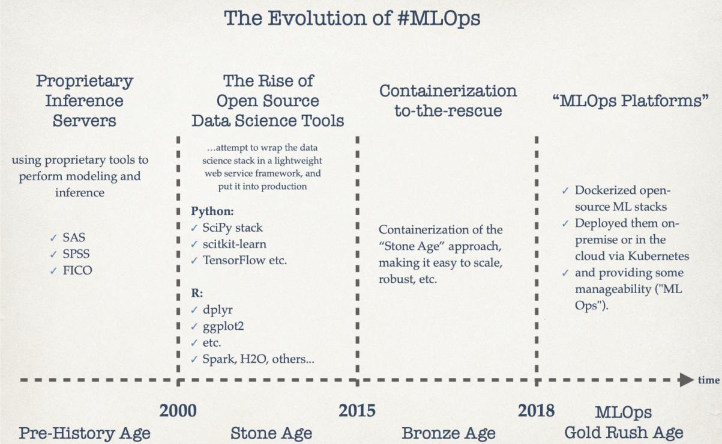
\includegraphics[width=1\textwidth]{evolucionTemporalMLOPS.png}
\label{fig:figura2}
\caption*{\footnotesize Fuente: \citet{visengeriyeva2020}}
\end{figure}


\newpage
La metodología MLOps es una disciplina que fusiona las mejores prácticas de desarrollo de software con los desafíos específicos del Machine Learning, con el objetivo de facilitar la implementación y gestión de modelos de aprendizaje automático. Con el auge del software de código abierto y la disponibilidad de datos, más profesionales de software comenzaron a usar bibliotecas Python o R para entrenar modelos ML. 

A medida que iba surgiendo la tecnología de contenerización, se resolvió el despliegue del modelo de forma escalable mediante el uso de contenedores Docker y Kubernetes. Recientemente, vemos la evolución de esas soluciones hacia plataformas de implementación de ML que cubren toda la iteración de experimentación, capacitación, implementación y monitoreo de modelos \citep{visengeriyeva2020}.
\newpage

\textbf{Proceso de la metodología MLOps}
\begin{itemize}
\item \textbf{Flujos de ML:} Los flujos de datos, también llamados pipelines de datos o procesos ETL (extraer, transformar y cargar), son procesos donde los datos son obtenidos desde una fuente, para ser transformada y luego cargada en la misma fuente o en otro sistema. Las transformaciones de los datos se refieren a todos los cambios necesarios sobre los mismos, para que queden con el formato que es requerido en el destino final (el modelo de ML).
\item \textbf{Versionado de modelos y de datos:} En aprendizaje automático es igual de importante mantener registro de las diferentes versiones del código, pero se le suma también la necesidad de registrar las versiones del modelo, así como de los datos que fueron utilizados para entrenarlo, y de otros datos como hiper-parámetros del modelo.
\item \textbf{Validación de modelos:} Se debe tener en cuenta:
    \begin{enumerate}
        \item \textbf{Precisión del modelo:} de los casos que el modelo clasificó como verdaderos positivos (TP).
        \item \textbf{Recall del modelo:} la precisión abierta por categorías.
        \item \textbf{Medición de sesgo en los datos:} es importante realizar mediciones que ayuden a entender si el modelo está sesgado.
        \item \textbf{Casos críticos:} un modelo puede tener buena precisión, exhaustividad(recall) y no estar sesgado, pero no tomar los casos más importantes en la historia reciente.
        \item \textbf{Medición de un modelo de regresión:}\\
- Métricas globales del modelo como RMSE, MAE Y R2.\\
- Las mismas métricas pero aperturadas por diferentes cortes, para entender si hay algún segmento en el cual el modelo tenga oportunidades de mejora.\\
- Medición del sesgo en los datos, igual que en los problemas de clasificación.\\
- Casos críticos, igual que en los problemas de clasificación.
    \end{enumerate}
\item \textbf{Validación de datos:} Se genera en dos pasos, el primero corresponde al más básico es la calidad de los mismos, lo cual incluye verificar cantidad de nulos, el SLA (service level agreement) de actualización de los datos, que todos los datos sean del tipo esperado, entre otros. El segundo es el más complejo consiste en monitorear la distribución de los datos. Un cambio en la distribución puede ser originada por una falla en alguno de los pipelines o por cambios en los datos \citep{rivero2022}. 
\end{itemize}


\subsection{Modelo de Machine Learning}

De acuerdo con Murphy (\citeyear{murphy2012}), el modelo Machine Learning se refiere a la localización automatizada de datos que se encuentran estandarizados, además es una herramienta constante en el proceso de extracción de grandes volúmenes de información para su organización y análisis, definido también como Big Data. En la actualidad el Machine Learning se encuentra en los motores de búsqueda con los cuales se desarrollan resultados instantáneos como por ejemplo los anuncios, software antispam, las transacciones con la tarjeta de crédito, etc.

Estas nuevas tecnologías, a través del internet, permiten la recopilación de bases de datos de un tamaño considerable, pueden ser históricos o datos en tiempo real, siendo posible el análisis de datos debido a las mejoras constantes en la tecnología y el desarrollo de software. Para Shalev y Ben (\citeyear{shalev2014}), este desarrollo ha permitido que las bases de datos se encuentren en distintos formatos, lo que es un desafío para orientar estrategias que permitan resolver distintos problemas de acuerdo a las necesidades de cada formato y de esta manera avanzar en el desarrollo de métodos para el Machine Learning.

El Machine Learning al ser un proceso automatizado que retoma patrones en grandes cantidades de datos, permitiendo la implementación de modelos que utilizan aplicaciones de análisis de datos predictivos, teniendo en cuenta:

    \begin{enumerate}
        \item Técnicas de aprendizaje automático siendo un modelo de la relación entre un conjunto de características descriptivas y una característica objetivo basado en un conjunto de ejemplos históricos o instancias comunes.
        \item Posteriormente, es posible con este modelo establecer nuevas predicciones de manera constante \citep{shalev2014}.
    \end{enumerate}

Por esta razón con el Machine Learning es posible establecer tres tipos de modelos el geométrico, el probabilístico y el lógico (ver tabla \ref{tab:modelos}) y tres tipos de aprendizajes: el supervisado, el no supervisado y semi-supervisado (ver tabla \ref{tab:tipos}), ya que se busca el aprendizaje continuo, conocer el progreso y la veracidad de la información que se desarrolla, porque:

\begin{quote}
    "Su aplicación está determinada en diferentes ámbitos dependiendo de las necesidades del problema, permitiendo a los científicos y especialistas tomar decisiones referentes a temas tan puntales como si un tipo de material puede ser separado por características de resistencia a la fragmentación o capacidad de absorción de energía pudiendo determinar con esto si es recomendable su uso en una u otra tarea específica" \citep[p.42]{salamanca2021}.
\end{quote}

\begin{table}[htbp]
\centering
\caption{Modelos para el desarrollo de Machine Learning}
\label{tab:modelos}
\begin{tabular}{|l|p{10cm}|}
\hline
\textbf{Modelo} & \textbf{Características} \\
\hline
Geométrico & El espacio de instancias es el conjunto de todas las instancias posibles o descriptibles, estén presentes en nuestro conjunto de datos o no. Por lo general, este conjunto tiene alguna estructura geométrica. Por ejemplo, si todas las características son numéricas, entonces se puede usar cada característica como una coordenada en un sistema de coordenadas cartesiano. \\
\hline
Probabilístico & Muchos de estos modelos se basan en la siguiente idea. Sea X las variables que se conoce por ejemplo, los valores de las características de nuestra instancia; y deje que, Y denote las variables de destino que nos interesan, por ejemplo, la clase de la instancia. La pregunta clave en el aprendizaje automático es cómo modelar la relación entre X e Y. \\
\hline
Lógico & Se inspira en la informática y la ingeniería. A este tipo lo llamo “lógico” porque los modelos de este tipo pueden traducirse fácilmente en reglas comprensibles para los humanos, como si \begin{verbatim}
if Viagra=1 then Class=Y=spam
\end{verbatim} \\
\hline
\end{tabular}
\caption*{\footnotesize Fuente: \citet{salamanca2021}}
\end{table}

\begin{table}[htbp]
\centering
\caption{Los tipos de aprendizaje en el ML}
\label{tab:tipos}
\begin{tabular}{|p{4cm}|p{10cm}|}
\hline
\textbf{Tipos} & \textbf{Fundamento} \\
\hline
Aprendizaje supervisado & Consiste en encontrar el mejor clasificador posible $f: X \rightarrow Y$ para un problema determinado. El algoritmo responsable de encontrar este mapeo se denomina algoritmo de clasificación, que infiere un modelo de cada ejemplo de entrada $x \in X$ y su respectiva clase $y \in Y$. Este modelo es una aproximación para la distribución de probabilidad conjunta (DPC) de las variables $X$ e $Y$. \\
\hline
Aprendizaje no supervisado & Son aquellos en los que no estamos interesados en ajustar pares (entrada, salida), sino en aumentar el conocimiento estructural de los datos disponibles (y posibles datos futuros que provengan del mismo fenómeno), por ejemplo, dando una agrupación de los datos según su similaridad (clustering), simplificando las estructura de los mismos manteniendo sus características fundamentales (como en los procesos de reducción de la dimensionalidad), o extrayendo la estructura interna con la que se distribuyen los datos en su espacio original (aprendizaje topológico). \\
\hline
Aprendizaje semi supervisado & El objetivo es la clasificación, pero la entrada contiene datos etiquetados y sin etiquetar. El aprendizaje semi-supervisado, debido a su estructura, se puede dividir principalmente en dos tipos, según el objetivo del análisis que se busque hacer a la base de datos:
\begin{minipage}[t]{\linewidth}
    \begin{enumerate}
      \item Aprendizaje transductivo, que separa el conjunto dado en conjunto de entrenamiento (donde la variable objetivo es conocida), y conjunto de prueba donde ésta no es dada.
      \item Aprendizaje inductivo trata de obtener una función de predicción usando todo el conjunto $\{(X, Y)\}$, es decir, usando tanto los datos donde la variable objetivo es conocida como aquellos en los que no.
    \end{enumerate}
\end{minipage} \\
\hline
\end{tabular}
\caption*{\footnotesize Fuente: \citet{salamanca2021}}
\end{table}

\newpage
Autores como \citet{contreras2022}, \citet{salamanca2021} y \citet{jara2016} explican que, en el campo del Machine Learning los métodos de predicción presentan un papel fundamental al permitir que las máquinas realicen predicciones precisas sobre datos no vistos. Existen varios métodos utilizados en el Machine Learning para generar predicciones, entre ellos se destacan los siguientes:

\begin{enumerate}
    \item Regresión: Es utilizado para predecir un valor numérico continuo basado en variables independientes. Algunos ejemplos comunes son la regresión lineal y la regresión logística, que se utilizan para predecir la relación entre variables \citep{salamanca2021}.
    \item Clasificación: Se utiliza para predecir la pertenencia a una clase o categoría específica. Los algoritmos de clasificación, como el árbol de decisiones, las máquinas de vectores de soporte (SVM) y los clasificadores de Naive Bayes, se emplean para clasificar datos en categorías predeterminadas \citep{salamanca2021}.
    \item Agrupamiento: Es utilizado para agrupar conjuntos de datos similares en clusters o grupos. Algunos métodos comunes de agrupamiento son el algoritmo k-means y el agrupamiento jerárquico, que ayudan a encontrar patrones y estructuras ocultas en los datos \citep{contreras2022}.
    \item Redes neuronales: Estas técnicas se basan en modelos inspirados en el funcionamiento del cerebro humano. Las redes neuronales profundas, como las redes neuronales convolucionales (CNN) y las redes neuronales recurrentes (RNN), han logrado grandes avances en áreas como la visión por computadora y el procesamiento del lenguaje natural \citep{salamanca2021}.
\end{enumerate}

Estos métodos de predicción en el Machine Learning han demostrado ser eficientes en una amplia gama de aplicaciones, desde la detección de fraudes hasta el diagnóstico médico y la recomendación de productos. La elección del método adecuado depende del tipo de datos, el problema a resolver y los objetivos específicos del proyecto de Machine Learning.


\subsubsection{Cultivo de aguacate Hass}

El cultivo del aguacate HASS es cada vez más popular en la agricultura debido a sus características y beneficios. El aguacate HASS es una variedad de aguacate que se distingue por su adaptabilidad a diferentes condiciones climáticas y su alta productividad. Según estudios realizados por el Departamento Administrativo de Nacional de Estadística \citep{dane2016cultivo}, esta variedad se ha destacado por su resistencia a enfermedades y plagas comunes en el cultivo del aguacate.

Una de las ventajas de cultivar el aguacate Hass es su capacidad para adaptarse a diferentes climas, según los autores \citet{reyes2022}, esta variedad es apta para regiones con temperaturas que oscilan entre los 10 y 35 grados Celsius, además, puede tolerar tanto condiciones secas como húmedas, lo que la convierte en una opción viable para diferentes áreas geográficas.

Cabe destacar, que  otra de las características  del aguacate Hass es su alta productividad, esta variedad puede alcanzar rendimientos superiores a los 20 kilogramos de fruta por árbol al año, esto la convierte en una opción rentable para los agricultores, ya que pueden obtener una mayor producción por unidad de superficie cultivada \citep{reyes2022}.

Además de su adaptabilidad y productividad, el aguacate Hass presenta resistencia a enfermedades comunes en el cultivo del aguacate, según los autores \citet{agapito2022}, esta variedad ha mostrado resistencia al hongo Phytophthora cinnamomi, causante de la pudrición de raíz, lo que reduce la necesidad de aplicar productos químicos para su control.

\subsubsection{Plagas Stenoma catenifer y heilipus lauri}

El cultivo del aguacate puede verse amenazado por diversas plagas que pueden afectar tanto las hojas, los frutos como las raíces de la planta, según  el Dane  (\citeyear{dane2016cultivo}) las plagas más comunes son el ácaro del aguacate entre los que se encuentran el Heilipus lauri y el Stenoma catenifer, quienes provoca un daño en la apariencia de la planta y puede reducir su capacidad de fotosíntesis, para controlar esta plaga, se pueden emplear insecticidas específicos o realizar una poda adecuada de las hojas afectadas.

Para \citet{carabali2022}, en el cultivo del aguacate Hass la Stenoma catenifer (ver figura \ref{fig:figuraStenoma}) desarrolla su polilla al alimentarse de los frutos del aguacate, perforando galerías y causando daños considerables en la calidad de la cosecha. Asimismo la plaga del barrenador del hueso del aguacate Heilipus spp (ver figura \ref{fig:figuraHeilipus}), puede causar daños graves al cultivo, las  larvas de este insecto se alimentan del interior del hueso del aguacate, lo que afecta el desarrollo adecuado del fruto \citep{carabali2022}.

\begin{figure}[h]
\centering
\caption{Fotografía del insecto Stenoma catenifer}
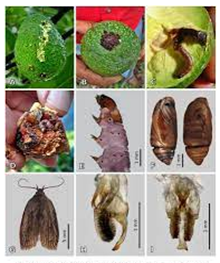
\includegraphics[width=0.5\textwidth]{stenoma.png}
\caption*{\footnotesize Fuente: \cite{diaz2017}}
\label{fig:figuraStenoma}
\end{figure}

\begin{figure}[h]
\centering
\caption{Fotografía del insecto Heilipus lauri}
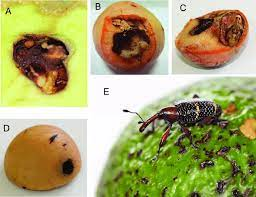
\includegraphics[width=0.5\textwidth]{heilipusLauri.png}
\caption*{\footnotesize Fuente: \cite{palacios2011}}
\label{fig:figuraHeilipus}
\end{figure}